\documentclass{beamer}
\usetheme{boxes}
\usecolortheme{sidebartab}
\usefonttheme{structureitalicserif}
\setbeamertemplate{bibliography item}{\insertbiblabel} % Removes the icon in references

\usepackage{graphicx}
\usepackage{siunitx}
\usepackage[version=3]{mhchem}

\title{A Scalable Database for Sensor Observations}

\author{Peter K. Kaiser, John N. Doe, \underline{Jutta Kaisaniemi}}

%\author{\texorpdfstring{Peter K. Kaiser\newline 
%Environmental Informatics Research Group, University of Zurich\newline
%\url{p.kaiser@example.org}}{Peter K. Kaiser}\newline
%\texorpdfstring{John N. Doe\newline
%Biogeochemistry Research Group, Australian National University\newline
%\url{j.doe@example.org}}{John N. Doe}\newline
%\texorpdfstring{\underline{Jutta Kaisaniemi}\newline
%College of Engineering and Computer Science, University of Eastern Finland\newline
%\url{j.kaisaniemi@example.org}}{Jutta Kaisaniemi}}

\date{\today}

\begin{document}

\maketitle
% \scriptsize\maketitle\normalsize

\begin{frame}
  \frametitle{Introduction}
  
  \begin{itemize}
  \item Of interest is CumulusRDF \cite{ladwig11cumulusrdf}
  \item Widely adopted in the literature \cite{phuoc11linked,lefort12qb}
  \end{itemize}
  
\end{frame}

\begin{frame}
  \frametitle{Introduction}
  
  \begin{itemize}
  \item Measure \ce{CO2}, \ce{CH4}, and \ce{H2O} fluxes
  \item Sampling frequency \SI{10}{\hertz} for \SI{30}{\minute}
  \end{itemize}
  
\end{frame}

\begin{frame}
  \frametitle{Results}
  
	\centering
	\begin{tabular}{|c|r|r|r|}
		\hline
    Subset & Observations & Triples & Distinct \\
  	\hline
  	30 m & \num{54000} & \num{810000} & \num{648007} \\
  	1 h & \num{108000} & \num{1620000} & \num{1296007} \\
  	\hline 
  \end{tabular}
  
\end{frame}

\begin{frame}
  \frametitle{Results}
  
  \centering
	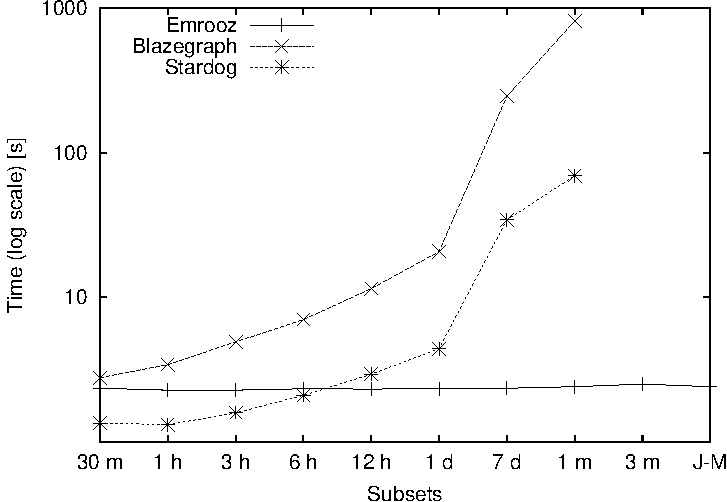
\includegraphics[scale=0.8]{query-performance-plot.pdf}
  
\end{frame}

\begin{frame}
  \frametitle{References}
  
  \tiny
  \bibliographystyle{plain} 
  \bibliography{bibliography}
  
\end{frame}

\end{document}